%!TEX root = Main.tex
\documentclass[Main]{subfiles}

\begin{document}
\section{Particle Filter} % (fold)
	\label{sec:particlefilter}
This lesson is about the Particle Filter. 
Particle Filters can be used for localization by spreading particles across the map and then use them as belief. 
This the last localization method presented in this course.

The basic idea with the particle filter in a localization application is to choose a number of particles, generate that many particles with random poses, and make them converges towards the actual position.
The basic algorithm is the following:
\begin{enumerate}
\item Generate a particle set $\chi$ of particles with random poses 
\item Calculate the importance weights of the particles 
\item Resample the particle set based on the importance weights
\item Move the particles
\item Go to step 2.
\end{enumerate}
In both \autoref{sec:localization} and \autoref{sec:kalman} there was the two state of operation; sensing and moving.
These two states also exists in the Particle Filter, where calculation of the importance weights and resampling matches sensing, and the movement of the particles matches the moving state.

In step 2 it can be seen that all the particles have their importance weight calculated at each iteration.
The importance weight is a measure of how well a particle matches the measured pose.
The weight can therefore be use as the belief of the robot pose.
It can for an example be calculated using a Gaussian distribution:
\begin{equation}
	p(\mathbf{x}|\mathbf{z}) = \frac{1}{\sqrt{2\pi^2 \cdot |\mathbf{C_z}|}} \exp \left( -\frac{1}{2}\cdot (\mathbf{z}-\mathbf{x})^T \mathbf{C_z}^{-1} (\mathbf{z}-\mathbf{x}) \right)
\end{equation}
Where $\mathbf{x}$ is a particles pose, $\mathbf{z}$ is the measured pose and $\mathbf{C_z}$ is the measurement noise.
By changing the measurement noise, the spread of the particles is also changed after resampling; the smaller the measurement noise, the smaller the spread.

Resampling is the part of the algorithm where the particles should converges towards the true robot pose.
The basic idea is that particles are chosen to be in the particle set, for the next iteration, with a probability which is proportional to the particles' importance weights.
There are different way to do resampling, but the method presented in this course is based upon the Low Variance Resampling algorithm.
This algorithm starts by sorting all the weights in the order of the particle index.
It then randomly select a particle, where all particles have the same probability of being selected.
\autoref{fig:low_var_resampling} is an example from \citep{Thrun2002} where the randomly selected particle is at index 6.
\begin{figure}[H]
	\centering
	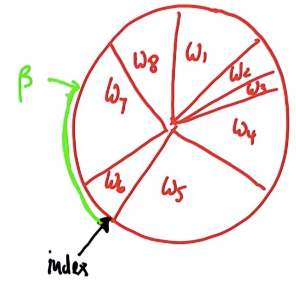
\includegraphics[width=0.3\linewidth]{./Figures/low_var_resampling.png}
	\caption{Low Variance Resampling example, borrowed from \citep{Thrun2015}}
	\label{fig:low_var_resampling}
\end{figure}\noindent
A $\beta$ value is created using the largest importance weight and some randomness, \autoref{eq:beta_calc}.
\begin{equation}
\label{eq:beta_calc}
	\beta = 2 \cdot w_{max} \cdot \mathcal{U}(0,1)
\end{equation}
The maximum weight is multiplied by $2$ to make it possible to "jump over" the particle with that weight.
The algorithm then checks if the $\beta$ value is larger than the weight at index i, $\beta > w_i$.
If this is the case, the weight is then subtracted from $\beta$ and the index is incremented, otherwise the particle at the index is added to the particle set for the next iteration. 
This process repeats until a particle is added to the set, and then repeats until a full set is created.
In this example $\beta$ is larger than $w_6$, so $\beta$ becomes $w_6$ smaller and the index become $7$.
$\beta$ is now smaller than $w_7$ which means that the particle at index $7$ is added to the next set. 
A new $\beta$ is then calculate and it continues from index $7$.
Using this algorithm insures a circular selection of the particles, where particles with high weight have a larger chance to be selected.
To summarize, the algorithm works in the following steps:
\begin{enumerate}
\item Randomly select an index where all particle have equal chance, $i = \mathcal{U}(1,N_{particles})$ 
\item Calculate $\beta$ based on the maximum weight, \autoref{eq:beta_calc}
\item Check if $\beta$ is larger than the weight at the index, $\beta > w_i$
\item If true
\begin{enumerate}
	\item Subtract the weight from $\beta$, $\beta = \beta-w_i$
	\item Increment the index, $i = i+1$
	\item Go to step 3	
\end{enumerate}
\item If false
\begin{enumerate}
	\item Add the particle to the particle set for the next iteration, $add \:\: particle_i \:\: to \:\: \chi_{k+1}$
	\item Go to step 2
\end{enumerate}
\end{enumerate}\fxnote{skal det være pseudokode istedet for?}
Now that the functionality of the particle filter have been described, an example of it is shown in \autoref{fig:pf_ex} where it is possible to see how the particles change over time.
\autoref{fig:pf_ex}a shows the initial particle set, where the height of the lines represent the importance weights. 
In \autoref{fig:pf_ex}b a measurement have been made and the importance weight have been updated.
Since the measurement shows a door, all the particles near door have a large weight compare to the rest.
\autoref{fig:pf_ex}c show the result after resampling and movement.
Notice how there are three larger densities of particles that matches the particles at the different doors after being moved.
\autoref{fig:pf_ex}d shows the particles after another measurement and weight update. And \autoref{fig:pf_ex}e is another resampling and movement.
From this it is obvious to see how the particles converges toward the robot position.

The last thing that will be described is the so called "kidnapped robot" situation.
This is where the particles converges toward a false pose, and the measurements suddenly does not match which means that the robot have no idea where it is since all the importance weight becomes small.
The basic particle filter cannot handle this situation, but it can easily be extended so it can.
One way to do it, is to only create, for an example, $90\%$ of the particle set from resampling and add $10\%$ newly generated particles.
The number of new particles can also be chosen dynamic, like it is in the Augmented Monte Carlo Localization algorithm which is described in details in \citep{Thrun2002}.
By adding new particles, there is a chance that one of these are near the true pose.
\begin{figure}[H]
	\centering
	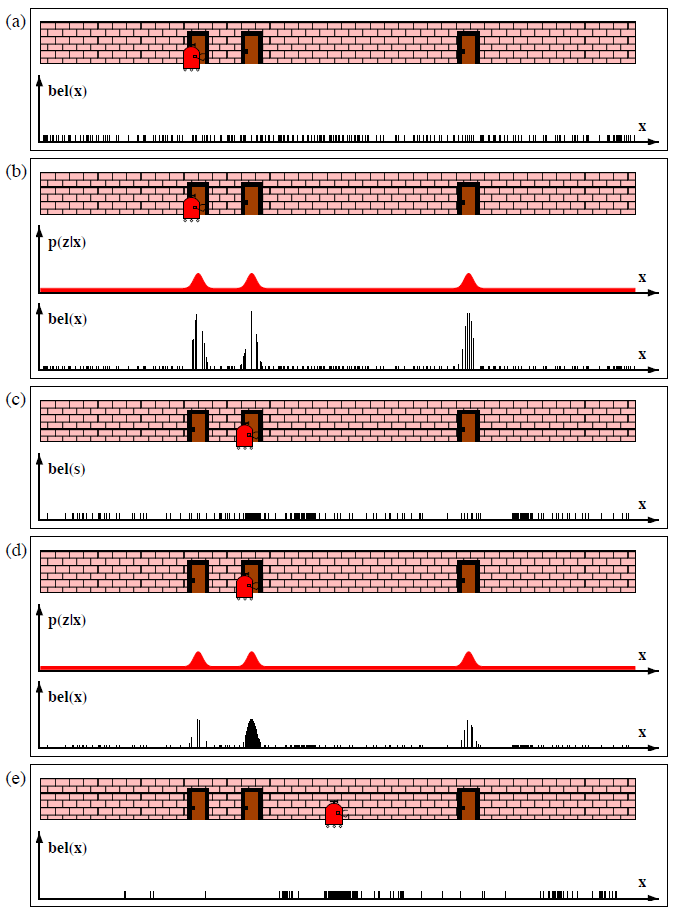
\includegraphics[width=1\linewidth]{./Figures/pf_ex.png}
	\caption{Particle filter example, borrowed from \citep{Thrun2002}}
	\label{fig:pf_ex}
\end{figure}\noindent
	% section introduction (end)

\end{document}